\documentclass[useAMS,usenatbib]{mn2e}
\usepackage[letterpaper,margin=0.65in]{geometry}
\usepackage[ansinew]{inputenc}
\usepackage{amsfonts}
\usepackage{amsmath}
\usepackage{graphicx}
\usepackage{epsfig}
\usepackage{color}
\usepackage{amssymb}
\usepackage[normalem]{ulem}
\usepackage{natbib}
\usepackage{url}

\def\aap{{ A\&A}}
\def\AaA{{ A\&A}}
\def\AJ{{AJ}}
\def\aj{{AJ}}
\def\ApJ{{ApJ}}
\def\apj{{ApJ}}
\def\apjl{{ApJL}}
\def\ApJL{{ApJL}}
\def\ApJSupp{{ApJS}}
\def\MN{{MNRAS}}
\def\mnras{{MNRAS}}
\def\pasp{{PASP}}
\def\jcap{JCAP}
\def\pasj{{PASJ}}
\def\nat{Nature}
\def\ARAA{{ARA\&A}}
\def\apjs{{ApJS}}
\def\araa{{ARA\&A}}
\def\apss{{Ap\&SS}}
\def\cjaa{{ChJAA}}
\def\aaps{{A\&AS}}

\newcommand{\eg}{{e.g., }}
\newcommand{\ie}{{i.e., }}

\title{A Hybrid Ensemble Learning Approach to Star-galaxy Classification}

\author[E. J. Kim et al.]{
  Edward J. Kim\thanks{jkim575@illinois.edu}$^1$, Robert J. Brunner$^2$,
  and Matias Carrasco Kind$^3$\\
$^1$Department of Physics, University of Illinois, Urbana, IL 61801 USA\\
$^2$Department of Astronomy, University of Illinois, Urbana, IL 61801 USA\\
$^3$National Center for Supercomputing Applications, Urbana, IL 61801 USA}

\begin{document}

\date{\today}

\pagerange{\pageref{firstpage}--\pageref{lastpage}} \pubyear{2015}

\maketitle

\label{firstpage}
\begin{abstract}
\textcolor{red}{Abstract goes here.}
\end{abstract}

\begin{keywords}
\textcolor{red}{keywords}
\end{keywords}


\section{Introduction}
  \label{section:introduction}

The problem of star-galaxy classification is fundamental to astronomy
and goes as far back as \cite{messier1781catalogue}.
A variety of different strategies have been developed 
to tackle this long-standing problem,
and yet it remains an unsolved challenge.
The most commonly used method to classify stars and galaxies
in large sky surveys is the morphological separation
~\citep{sebok1979optimal, kron1980photometry, valdes1982resolution,
yee1991faint, vasconcellos2011decision,
henrion2011bayesian}.
It relies on the assumption that
stars appear as point sources
while galaxies appear as resolved sources.
However,
currently ongoing and upcoming large photometric surveys,
such as the Dark Energy Survey
(DES\footnote{http://www.darkenergysurvey.org/})
and the Large Synoptic Survey Telescope
(LSST\footnote{http://www.lsst.org/lsst/}),
will detect a vast number of unresolved galaxies
at faint magnitudes.
Near a survey's limit, the photometric observations
cannot reliably separate stars from unresolved galaxies
by morphology alone without leading to
incompleteness and contamination in the star and galaxy samples.

The contamination of unresolved galaxies can be mitigated
by using training based algorithms.
Machine learning methods have the advantage that
it is easier to include extra information,
such as concentration indices, shape information,
or different model magnitudes.
However,
they are only reliable within the limits of the training data,
and it can be difficult to extrapolate these algorithms
outside the parameter range of the training data.
These techniques can be further categorized into
supervised and unsupervised learning approaches.

In supervised learning, 
the input attributes (\eg magnitudes or colors)
are provided along with the truth labels (\eg star or galaxy).
\cite{odewahn1992automated} pioneered
the application of neural networks
to the star-galaxy classification problem,
and it has become a core part of
the astronomical image processing software
\textsc{SExtractor}~\citep{bertin1996sextractor}.
Other successfully implemented examples include
decision trees~\citep{weir1995automated, suchkov2005census, ball2006robust}
and Support Vector Machines~\citep{Fadely2012}.
Unsupervised machine learning techniques
are less common
as they do not utilize the truth labels during the training process
and only the input attributes are used.

Physically based template fitting methods
have also been used for the star-galaxy classification
problem~\citep{robin2007stellar, Fadely2012}.
Template fitting approaches infer a source's properties
by finding the best match between
the measured set of magnitudes (or colors)
and the synthetic set of magnitudes (or colors)
computed from a set of spectral templates.
Although it is not necessary to obtain
a high-quality spectroscopic training sample,
these techniques do require
a representative sample of theoretical or empirical templates
that span the possible spectral energy distributions (SEDs)
of stars and galaxies.
Furthermore, they are not exempt from uncertainties
due to measurement errors on the filter response curves,
or from mismatches between the observed magnitudes
and the template SEDs.

In this paper,
we present a novel star-galaxy classification framework
that combines and fully exploits different classification techniques
to produce a more robust classification.
In particular,
we show that the combination of a morphological separation method,
a template fitting technique, a supervised machine learning method,
and an unsupervised machine learning algorithm
can improve the overall performance over any individual method.
In Section~\ref{section:classification_methods},
we describe each of the star-galaxy classification methods.
In Section~\ref{section:classification_combination_methods},
we describe different classification combination techniques
In Section~\ref{section:data},
we describe the Canada-France Hawaii Telescope Lensing Survey (CFHTLenS)
data set with which we test the algorithms.
In Section~\ref{section:results_and_discussion},
we compare the performance of our combination techniques
to the performance of the individual classification techniques.

\section{Classification Methods}
  \label{section:classification_methods}

In this section, we present
four distinct star-galaxy classification techniques.
The first method is
a supervised machine learning technique named \texttt{TPC}
(Trees for Probabilistic Classification),
which uses prediction trees and a random forest~\citep{carrascokind2013tpz}.
The second method is
an unsupervised machine learning technique named \texttt{SOMc},
which uses self-organizing maps (SOM) and a random atlas
to provide a classification~citep{carrascokind2014somz}.
The third method is
a Hierarchical Bayesian template fitting technique
based on the work by \cite{Fadely2012},
which fits SED templates from star and galaxy libraries
to an observed set of measured flux values.
The fourth method is a morphological separation method,
which uses a hard cut in the half-light radius vs.\ magnitude plane.

Collectively, these four methods represent the majority of all
standard star-galaxy classification approaches published in the literature.
It is very likely that any new classification technique would be
functionally similar to one of these four   methods.
Therefore, any of these four methods could in principle be replaced by a similar method. 


\subsection{Morphological Separation}

The simplest and perhaps the most widely used approach
to star-galaxy classification is
to make a hard cut in the space of photometric attributes.
As a first-order morphological selection of point sources,
we adopt a technique that is popular among the weak lensing 
community~\citep{Kaiser1995}.
As Figure~\ref{fig:morph} shows, there is a distinct locus
produced by point sources in the half-light radius
($r_h$; estimated by \textsc{SExtractor}'s \texttt{FLUX\_RADIUS} parameter)
vs.\ the $i$-band magnitude plane.
A rectangular cut in this size-magnitude plane separates point sources,
which are presumed to be stars,
from resolved sources,
which are presumed to be galaxies.
The boundaries of the selection box are determined by
manually inspecting the size-magnitude diagram.


\begin{figure}
  \centering
  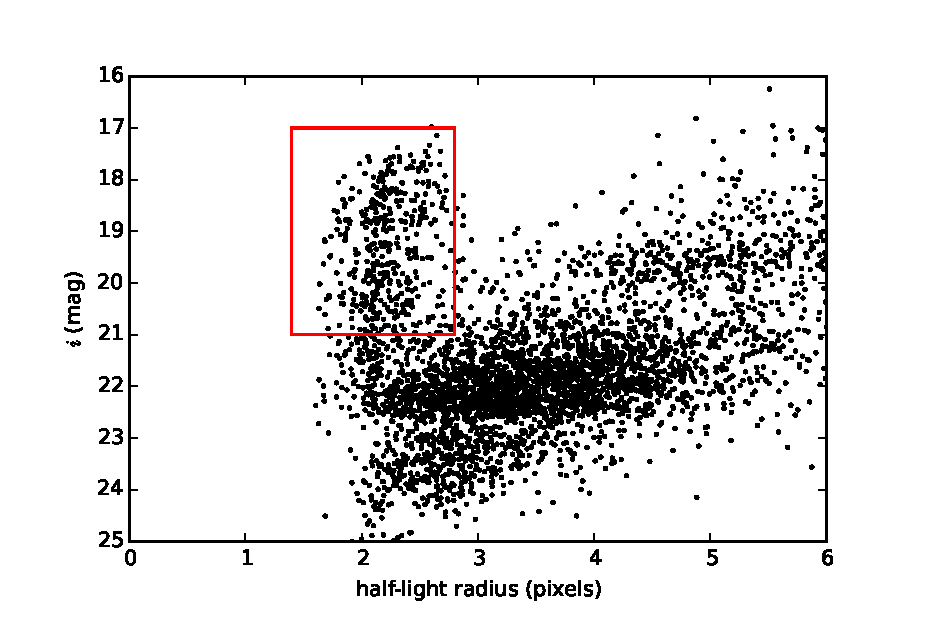
\includegraphics[width=0.95\linewidth]{figures/morph.eps}
  \caption{Half-light radius ($r_h$) vs.\ magnitude.}
  \label{fig:morph}
\end{figure}


One of the disadvantages of such cut-based methods is
that it classifies every source with absolute certainty.
It is difficult to justify such a decisive classification
near a survey's magnitude limits,
where measurement uncertainties generally increase.
A more informative approach is to provide probabilistic classifications.
Although a recent work by \cite{henrion2011bayesian}
implemented a probabilistic classification using a Bayesian approach
on the morphological measurements alone,
here we use a cut-based morphological separation
to demonstrate the advantages of our combination techniques.
In particular, we later show that
the binary output (\ie 0 or 1) of cut-based methods
can be transformed into a
probability estimate by combining them
with the probability outputs from other
probabilistic classification techniques,
such as \texttt{TPC}, \texttt{SOMc}, and \texttt{HB}.


\subsection{Supervised Machine Learning: TPC}

\texttt{TPC} is a parallel, supervised machine learning algorithm
that uses prediction trees and random forest 
techniques~\citep{breiman1984classification, breiman2001random}
to produce star-galaxy classification.
\texttt{TPC} is a part of a publicly available software package called
\texttt{MLZ}\footnote{http://lcdm.astro.illinois.edu/code/mlz.html}
(Machine Learning for Photo-$z$).
The full software package includes, among other capabilities,
\texttt{TPZ}, a supervised photo-$z$ technique
\citep[regression mode;][]{carrascokind2013tpz},
\texttt{TPC}, a supervised star-galaxy classification technique
(classification mode),
\texttt{SOM}$z$, an unsupervised photo-$z$ technique
\citep[regression mode;][]{carrascokind2014somz},
and
\texttt{SOMc}, an unsupervised star-galaxy classification technique
(classification mode).

\texttt{TPC} uses classification trees,
a type of prediction trees that are designed to
provide a classification or predict a discrete category.
Prediction trees are built by asking a sequence of questions
that recursively split the data into branches
until a terminal leaf is created
that meets a stopping criterion
(\eg a minimum leaf size).
The optimal split dimension is decided by
choosing the attribute that maximizes
the \textit{Information Gain} ($I_G$), which is defined as

\begin{equation}
  I_G \left(D_{\mathrm{node}}, X\right)
  = I_d \left( D_{\mathrm{node}} \right)
  - \sum_{x \in \mathrm{values}(X)}
  \frac{|D_{\mathrm{node}, x}|}{|D_{\mathrm{node}}|}
  I_d \left( D_{\mathrm{node}, x} \right),
  \label{eq:information_gain}
\end{equation}

\noindent
where $D_{\mathrm{node}}$ is the training data in a given node,
$X$ is one of the possible dimensions (\eg magnitudes or colors)
along which the node is split, and
$x$ are the possible values of a specific dimension $X$.
$|D_{\mathrm{node}}|$ and $|D_{\mathrm{node}, x}|$ are the size of the total training data
and the number of objects in a given subset $x$ within the current node,
respectively.
$I_d$ is the impurity degree index,
and \texttt{TPC} can calculate $I_d$
from any of the three standard different impurity indices:
\textit{information entropy}, \textit{Gini impurity},
and \textit{classification error}.
Here, we use the information entropy,
which is defined similarly to the thermodynamic entropy:

\begin{equation}
  I_d \left( D \right)
  = - f_g \log_{2} f_g - (1 - f_g) \log_{2} f_g,
\end{equation}

\noindent
where $f_g$ is the fraction of galaxies in the training data.
At each node in our tree,
we scan all dimensions to identify the split point that
maximizes the information gain as defined by Equation~\ref{eq:information_gain},
and select the attribute that maximizes the impurity index overall.

In a technique called random forest,
we create bootstrap samples
(\ie $N$ randomly selected objects with replacement)
from the input training data
by sampling repeatedly from the magnitudes using the magnitude errors.
We use these bootstrap samples to construct
multiple, uncorrelated prediction trees
whose individual predictions are aggregated to produce
a star-galaxy classification for each source.

We also use a cross validation technique called
Out-of-Bag~\citep[OOB;][]{breiman1984classification, carrascokind2013tpz}.
When a tree (or a map) is built in \texttt{TPC} (or \texttt{SOMc}),
a fraction of the training data, usually one-third,
is left out and not used in training the trees or maps.
After a tree is constructed using two-thirds of the training data,
the final tree is applied to the remaining one-third
to make a classification.
This process is repeated for every tree,
and the predictions from each tree are aggregated
for each object to make the final star-galaxy classification.
We emphasize that if an object is used for training a given tree,
it is never used for subsequent prediction by that tree.
Thus, the OOB data is an unbiased estimation of the errors
and can be used as cross-validation data
as long as the OOB data remain similar to the final test data set.
The OOB technique can also provide extra information such as
a ranking of the relative importance of the input attributes
used in the prediction.
The OOB technique can prove extremely valuable
when calibrating the algorithm,
when deciding which attributes to incorporate in the construction of the trees,
and when combining this approach with other techniques.


\subsection{Unsupervised Machine Learning: SOMc}

A Self-Organizing Map
\citep[SOM;][]{kohonen1990self, kohonen2001self}
is an unsupervised, artificial neural network algorithm
that is capable of projecting high-dimensional input data
onto a low-dimensional map
through a process of competitive learning.
In astronomical applications,
the high-dimensional input data can be
magnitudes, colors, or some other photometric attributes.
The output map is usually chosen to be two-dimensional
for the visualization.
The differences between a SOM and other neural network algorithms are
that a SOM is unsupervised,
there are no hidden layers and therefore no extra parameters,
and it produces a direct mapping
between the training set and the output network.
In fact, a SOM can be viewed as a non-linear generalization
of a principal component analysis (PCA) algorithm.

The key characteristic of SOM is that
it retains the topology of the input training set,
revealing correlations between input data that are not obvious.
The method is unsupervised:
the user is not required to specify the desired output
during the creation of the lower-dimensional map,
and the mapping of the components from the input vectors
is a natural outcome of the competitive learning process.

During the construction of a SOM,
each node on the two-dimensional map is represented by
weight vectors of the same dimension
as the number of attributes used to create the map itself.
In an iterative process,
each object in the input sample is individually used
to correct these weight vectors.
This correction is determined so that the specific neuron (or node),
which at a given moment best represents the input source,
is modified along with the weight vectors
of that node's neighboring neurons.
As a result, this sector within the map
becomes a better representation of the current input object.
This process is repeated for every object in the training data,
and the entire process is repeated for several iterations.
Eventually, the SOM converges to its final form where
the training data is separated into groups of similar features.

In a similar approach to random forest in \texttt{TPZ} and \texttt{TPC},
\texttt{SOM}$z$ uses a technique called \textit{random atlas}
to provide photo-$z$ estimation \citep{carrascokind2014somz}.
In random atlas, the prediction trees of random forest are replaced by maps,
and each map is constructed from different bootstrap samples
of the training data.
Furthermore, we create random realizations of the training data
by perturbing the input attributes by their measurement error.
For each map, we can either use all available attributes,
or randomly select a subsample of the attribute space.
This SOM implementation can also be
applied to the classification problem,
and we refer to it as \texttt{SOMc}
in order to differentiate it from 
the photo-$z$ estimation problem (regression mode).
We also use the random atlas approach
in some of the classification combination approaches as discussed in
Section~\ref{section:classification_combination_methods}.

One of the most important parameter in \texttt{SOMc}
is the topology of the two-dimensional SOM,
which can be rectangular, hexagonal, or spherical.
To classify stars and galaxies in the CFHTLenS data,
we use a spherical topology,
which is constructed by using
\texttt{HEALPIX}~\citep{gorski2005healpix}.
Furthermore, similar to \texttt{TPC},
we use the OOB technique to make an unbiased estimation of errors.
For a complete description of the SOM implementation
and its application to the estimation of
photo-$z$ probability distribution functions,
we refer the reader to \cite{carrascokind2014somz}.

\subsection{Template fitting: Hierarchical Bayesian}

One of the most common methods to classify a source
based on its observed magnitudes is template fitting.
Template fitting algorithms do not require a spectroscopic training sample;
there is no need for additional knowledge outside the
observed data and the template SEDs.
However, any incompleteness in our knowledge of the template SEDs
that fully span the possible SEDs of observed sources
may lead to misclassification of sources.

Bayesian algorithms use Bayesian inference to quantify
the relative probability that each template matches
the input photometry
and determines a probability estimate by computing
the posterior that a source is a star or a galaxy.
In this work, we have modified and parallelized
a publicly available Hierarchical Bayesian (HB) template fitting
algorithm by \cite{Fadely2012}.
In this section, we provide a brief description
of the HB template fitting technique;
for the details of the underlying HB approach,
we refer the reader to \cite{Fadely2012}.

We write the posterior probability that a source is a star as

\begin{equation}
P \left( S | \mathbf{x}, \mathbf{\theta} \right)
= P \left( \mathbf{x} | S, \mathbf{\theta} \right)
P \left( S | \mathbf{\theta} \right),
\end{equation}

\noindent
where $\mathbf{x}$ represents a given set of observed magnitudes,.
We have also introduced the \textit{hyperparameter} $\mathbf{\theta}$,
a nuisance parameter that characterizes our uncertainty
in the prior distribution.
To compute the likelihood that a source is a star,
we marginalize over all star and galaxy templates $\mathbf{T}$.
In a template-fitting approach,
we marginalize by summing up
the likelihood that a source has the set of magnitudes $\mathbf{x}$
for a given star template
as well as the likelihood for a given galaxy template:

\begin{equation}
  P \left(\mathbf{x} | S, \mathbf{\theta} \right)
  = \sum_{t \in \mathbf{T}}
  P \left(\mathbf{x} | S, t, \mathbf{\theta} \right)
  P \left(t | S, \mathbf{\theta} \right).
  \label{eq:marginalize_template}
\end{equation}

\noindent
The likelihood of each template
$P \left( \mathbf{x} | S, \mathbf{\theta} \right)$
is itself marginalized over the uncertainty
in the template-fitting coefficient.
Furthermore, for galaxy templates, we introduce another step that 
marginalizes the likelihood by redshifting a given galaxy template
by a factor of $1 + z$.

Marginalization in Equation~\ref{eq:marginalize_template}
requires that we specify the prior probability
$P \left(t | S, \mathbf{\theta} \right)$
that a source has spectral template $t$ (at a given redshift).
Thus, the probability that a source is a star (or a galaxy)
is either the posterior probability itself
if a prior is used,
or the likelihood itself if an uniformative prior is used.
In a Bayesian analysis, it is preferable to use a prior,
which can be directly computed either from physical assumptions,
from an empirical function calibrated by
using a spectroscopic training sample,
or from an empirical function calibrated by
using machine learning techniques.
In an HB approach, the entire sample of sources is used to
infer the prior probabilities for each individual source.

Since the templates are discrete in both SED shape and physical properties,
we parametrize the prior probability of each template
as a discrete set of weights such that

\begin{equation}
\sum_{t \in \mathbf{T}}
P \left(t | S, \mathbf{\theta} \right) = 1.
\end{equation}

\noindent
These weights correspond to the hyperparameters,
which can be inferred by sampling
the posterior probability distribution in the hyperparameter space.
For the sampling, we use \texttt{emcee}, a Python implementation of the
affine-invariant Markov Chain Monte Carlo (MCMC) ensemble sampler~\citep{Foreman-Mackey2013}.  

As the goal of template fitting methods is to minimize
the difference between observed and theoretical magnitudes,
this approach heavily relies on
both the use of SED templates and
the accuracy of the transmission functions
for the filters used for particular survey.
For our stellar templates,
we use the empirical SED library from \cite{pickles1998stellar}.
The Pickles library consists of 131 stellar templates,
which span all normal spectral types
and luminosity classes at solar abundance,
as well as metal-poor and metal-rich F-K dwarf 
and G-K giant and supergiant stars.
\textcolor{blue}{
We supplement the stellar library with
100 SEDs from \cite{chabrier2000evolutionary},
which include low mass stars and brown dwarfs
with different $T_{eff}$ and surface gravities.
We also include four white dwarf templates of
\cite{bohlin1995white}.
}
For our galaxy templates,
we use the four CWW spectra from \cite{coleman1980colors},
which include an Elliptical, an Sba, an Sbb,
and an Irregular galaxy template.
When extending an analysis to higher redshift,
the CWW library is often augmented with
two star bursting galaxy templates from \cite{kinney1996template}.
\textcolor{blue}{
From the six original CWW and Kinney spectra,
intermediate templates are created by interpolation
for a total of 51 SEDs.
}

All of the above templates are convolved
with the filter response curves to generate model magnitudes.
These response curves consist of
$u$, $g$, $r$, $i$, $z$ filter transmission functions
for the observations taken by the
Canada-France Hawaii Telescope (CFHT).


\section{Classification combination methods}
  \label{section:classification_combination_methods}

Building on the work in the field of ensemble learning,
we combine the predictions from
individual star-galaxy classification techniques
using ensemble learning techniques known as
Bayesian Model Combination (BMC)
and a variant of an ensemble learning technique known as stacking.
The main idea behind ensemble learning is to weigh
the predictions from individual models
and combine them to obtain a prediction
that outperforms every one of 
them individually~\citep{rokach2010ensemble}.

\subsection{Unsupervised Binning}
  \label{section:random_atlas}

Given the variety of star-galaxy classification methods
we are using,
we fully expect the relative performance
of the individual techniques to vary across
the parameter space spanned by the data.
For example, it is reasonable to expect 
supervised techniques to outperform other techniques
in areas of parameter space that are well-populated
with training data.
Similarly, we can expect unsupervised approaches
such as \texttt{SOM} or template fitting approaches 
to generally perform better when training data
is either sparse or unavailable.

We therefore adopt the binning strategy similar to 
\cite{carrascokind2014exhausting}.
In this binning strategy,
we allow different classifier combinations 
in different parts of parameter space
by creating two-dimensional SOM representations of
the full nine-dimensional magnitude-color space:
$u$, $g$, $r$, $i$, $z$, $u-g$, $g-r$, $r-i$, and $i-z$.
A SOM representation can be rectangular, hexagonal, or spherical;
here we choose a 10$\times$10 rectangular topology to facilitate 
visualization as shown in Figure.~\ref{fig:som_colors}.
For all combination methods,
we use only the OOB (cross validation) data contained in each cell
to compute the relative weights for the base classifiers.
The weights within individual cells are then applied to the test data
to make the prediction.

Furthermore, we construct a collection of SOM representations
and subsequently combine the predictions from each map
into a meta-prediction.
Given a training sample of $N$ sources,
we generate $N_R$ random realizations of training data
by perturbing the attributes
with the measured uncertainty for each attribute.
The uncertainties are assumed to be normally distributed.
In this manner,
we reduce the bias towards the data
and introduce randomness in a systematic manner.
For each random realization of a training sample,
we create $N_M$ bootstrap samples of size $N$
to generate $N_M$ different maps.

After all maps are built,
we have a total of $N_R \times N_M$ probabilistic outputs
for each of the $N$ sources.
To produce a single probability estimate for each source,
one can take the mean, the median, or some other simple statistic.
With a sufficient number of maps,
we find that there is usually negligible difference
between taking the mean and taking the median,
and so we use the median in the following sections.
We note that it is also possible to establish confidence intervals
using the distribution of the probability estimates.

\subsection{Weighted Average}

The simplest approach to combine different combination techniques is
to simply add the individual classifications from the base classifiers
and renormalize the sum.
In this case, the final probability is given by
\begin{equation}
P\left(S | \mathbf{x}, \mathbf{M} \right)
= \sum_{i} P \left( S | \mathbf{x}, M_{i} \right),
\end{equation}

\noindent
where $\mathbf{M}$ is the set of models
(\texttt{TPC}, \texttt{SOMc}, \texttt{HB}, and morphological separation
in our work).
We improve on this simple approach
by using the binning strategy to
calculate the weighted average of each bin separately,
rather than globally.


\subsection{Bucket of Models (BoM)}

After the multi-dimensional input data have been binned,
we can use the cross-validation data
to choose the best model within each bin,
and we use only that model within that specific bin
to make predictions for the test data.
We use the mean squared error
(MSE; also known as Brier score~\citep{brier1950verification})
as a classification error metric. We define MSE as

\begin{equation}
  \mathrm{MSE} = \frac{1}{N} \sum^{N - 1}_{i = 0}
  \left( y_i - \hat{y}_i \right)^2,
  \label{eq:mse}
\end{equation}

\noindent
where $\hat{y}_i$ is the actual truth value
(\eg 0 or 1) of the $i^{\text{th}}$ data, 
and $y_{i}$ is the probability prediction made by the models.
Thus, a model with the minimum MSE is chosen in each bin
and is assigned a weight of one,
and zero for all other models.
However, the chosen model is allowed to vary between different bins.

\subsection{Stacking}

Instead of selecting a single model that performs best within each bin,
we can train a learning algorithm to combine the output values of
several other base classifiers in each bin.
An ensemble learning method of using a meta-classifier
to combine lower-level classifiers is known as \textit{stacking}
or \textit{stacked generalization}~\citep{wolpert1992stacked}.
Although any arbitrary algorithm
can theoreticaly be used as a meta-classifier,
a logistic regression or a linear regression is often used
in practice.
In our work,
we use a single-layer multi-response linear regression algorithm,
which often shows the best performance~\citep{breiman1996stacked, ting1999issues}.


\subsection{Bayesian Model Combination}

We also use a model combination technique \citep{Monteith2011} known as
Bayesian Model Combination (BMC).
BMC uses Bayesian principles to generate an ensemble combination of
different classifiers~\citep{Monteith2011}.
The posterior probability that a source is a star is given by

\begin{equation}
  P \left(S | \mathbf{x}, \mathbf{D}, \mathbf{M}, \mathbf{E} \right)
  = \sum_{e \in \mathbf{E}} P \left(S | \mathbf{x}, \mathbf{M}, e \right)
  P \left(e | \mathbf{D} \right),
  \label{eq:p_star_bmc}
\end{equation}

\noindent
where $\mathbf{D}$ is the data set,
and $e$ is an element in the ensemble space $\mathbf{E}$ of possible model combinations.
By Bayes' Theorem, the posterior probability of $e$ given $\mathbf{D}$ is given by

\begin{equation}
  P \left(e | \mathbf{D} \right)
  = \frac{P \left(e \right)}{P \left(\mathbf{D} \right)}
  \prod_{d \in \mathbf{D}} P \left( d | e \right)
  \propto P \left(e\right) \prod_{d \in \mathbf{D}} P \left(d | e \right).
  \label{eq:p_ensemble}
\end{equation}

\noindent
Here, the product of $P\left(d \mid e\right)$ is
over all individual data $d$ in the training data $\mathbf{D}$,
and $P\left(\mathbf{D}\right)$ is merely a normalization factor
and not important.

For binary classifiers whose output is either zero or one
(\eg a cut-based morphological separation),
we assume that each example is corrupted with
an average error rate $\epsilon$.
This means that
$P\left(d|e\right) = 1-\epsilon$ if the combination $e$
correctly predicts class $\hat{y}_i$ for the $i^{\text{th}}$ object,
and $P\left(d|e\right) = \epsilon$ if it predicts an incorrect class.
The average rate $\epsilon$ can be estimated by
the fraction $\left(M_g + M_s\right) / N$,
where $M_g$ is the number of true galaxies classified as stars,
$M_s$ is the number of true stars classified as galaxies,
and $N$ is the total number of sources.
Equation~\ref{eq:p_ensemble} then becomes

\begin{equation}
  P \left( e | \mathbf{D} \right) \propto 
  P \left( e \right) \left(1 - \epsilon \right)^{N_s + N_g}
  \left( \epsilon \right)^{M_s + M_g}.
\end{equation}

\noindent
For probabilistic classifiers,
we can directly use the probabilistic predictions
and write Equation~\ref{eq:p_ensemble} as

\begin{equation}
  P \left( e | \mathbf{D} \right) \propto 
  P \left( e \right) \prod_{i=0}^{N-1}
  \hat{y}_i y_i + 
  \left(1 - \hat{y}_i\right) \left(1 - y_i\right).
\end{equation}


Although the space $\mathbf{E}$ of potential model combinations
is in principle infinite,
we can produce a reasonable finite set
of potential model combinations by using sampling techniques.
In our implementation,
the weights of each combination of the base classifiers
is obtained by sampling from a Dirichlet distribution.
We first set all alpha values of a Dirichlet distribution.
We then sample this distribution $q$ times
to obtain $q$ sets of weights.
For each combination,
we assume a uniform prior and
calculate $P\left(e|\mathbf{D}\right)$ using Equation~\ref{eq:p_ensemble}.
We select the combination with the highest $P\left(e|\mathbf{D}\right)$,
and update the alpha values by
adding the weights of the most probable combination
to the current alpha values.
The next $q$ weight sets of weights are drawn
using the updated alpha values.

We continue the sampling process until
we reach a predefined number of combinations,
and finally use Equation~\ref{eq:p_star_bmc} to compute
the posterior probability that a source is a star (or a galaxy).
In this paper, we use a $q$ value of three,
and 1,000 model combinations were considered.


We also use a binned version of the BMC technique,
where we use a SOM representation
to apply different model combinations
for different regions of the parameter space.
We however note that introducing randomness
though the construction of different SOM representations
does not show significant
improvement over using only one single SOM representation.
This similarity is likely due to the randomness 
that has already been introduced by 
the sampling from the Dirichlet distribution.
Thus, our BMC technique uses one SOM,
while other base models (WA, BoM, and stacking)
generate $N_R$ random realizations of $N_M$ maps.


\section{Data}
  \label{section:data}

We use photometric data from
the Canada-France-Hawaii Telescope Lensing Survey
\cite[CFHTLenS\footnote{http://www.cfhtlens.org/};][]
{Heymans2012,Erben2013,Hildebrandt2012}.
This catalog consits of more than twenty five million objects
with a limiting magnitude of $i_{\text{AB}} \approx 25.5$. 
It covers a total of 154 square degrees
in the four fields of CFHT Legacy Survey~\citep[CFHTLS;][]{gwyn2012canada}
observed in the five photometric bands:
$u$, $g$, $r$, $i$, and $z$.

We have cross-matched reliable spectroscopic galaxies from
the Deep Extragalactic Evolutionary Probe Phase 2~
\citep[DEEP2;][]{Davis2003,Newman2013a},
the Sloan Digital Sky Survey Data Release 10~\citep[SDSS-DR10]{Ahn2014},
the VIsible imaging Multi-Object Spectrograph (VIMOS)
Very Large Telescope (VLT) Deep Survey~
\citep[VVDS;][]{LeFevre2005,Garilli2008}, and
the VIMOS Public Extragalactic Redshift Survey~\citep[VIPERS;][]{Garilli2014},
In the end, we have 8,545 stars and 57,843 galaxies available
for the training and testing processes.

Our goal here is not to obtain the best classifier
performance; for this we would have fine tuned individual base
classifiers and chosen sophisticated models best suited to the
particular properties of the CFHTLenS data.
For example, \cite{Hildebrandt2012} suggest that
all objects with $i > 23$ in the CFHTLenS dataset
may be classified as galaxies
without significant incompleteness in the galaxy sample.
Although this approach works because
the high Galactic latitude fields of the CFHTLS contain
relatively few stars,
it is very unlikely that such an approach
will meet the science requirements for the quality of
star-galaxy classification in lower latitude, star-crowded fields.
Rather, our goal for the CFHTLenS dataset
is to demonstrate the usefulness
of combining different classifiers even when
the base classifiers may be poor or trained on partial data.

\section{Results and Discussion}
  \label{section:results_and_discussion}

In this section, we present the classification performance of
the four different combination techniques,
as well as the individual star-galaxy classification techniques
on the CFHTLenS test data.


\subsection{Classification Metrics}

Probabilistic classification models can be considered as
functions that output a probability estimate of each source
to be in one of the classes (\eg a star or a galaxy).
Although the probability estimate can be used as a weight 
in subsequent analyses to improve or enhance
a particular measurement~\citep{ross2011ameliorating},
it can also be converted into a class label
by using a threshold (probability cut).
The simplest way to choose the threshold is to set it to a fixed value,
\eg $p_\mathrm{cut} = 0.5$.
This is, in fact, what is often done
\citep[\eg][]{henrion2011bayesian, Fadely2012}.
However, choosing $0.5$ as a threshold is not the best choice
for an unbalanced data set, where galaxies outnumber stars.
Furthermore, setting a fixed threshold ignores the operating condition 
(\eg science requirements, stellar distribution, misclassification costs)
where the model will be applied.


When we have no information about the operating condition
when evaluating the performance of classifiers,
there are effective tools such as
the Receiver Operating Characteristic (ROC) curve
\citep{swets2000better}.
An ROC curve is a graphical plot that illustrates the true positive rate
versus the false positive rate of a binary classifier
as its classification threshold (probability cut) is varied.
The Area Under the Curve (AUC) summarizes the curve information
in a single number,
and can be used as an assessment of the overall performance.

In astronomical applications,
the operating condition usually translates to
the completeness and purity requirements of the star/galaxy sample,
We define the galaxy \textit{completeness}
$c_g$ (also known as recall or sensitivity) as
the fraction of the number of true galaxies classified as galaxies
out of the total number of true galaxies,
\begin{equation}
c_g = \frac{N_g}{N_g + M_g},
\end{equation}

\noindent
where $N_g$ is the number of true galaxies classified as galaxies
and $M_g$ is the number of true galaxies classified as stars.
We define the galaxy \textit{purity} $p_g$ (also known as precision
or positive predictive value)
as the fraction of the number of true galaxies classified as galaxies
out of the total number of objects classified as galaxies, 
\begin{equation}
p_g = \frac{N_g}{N_g + M_s},
\end{equation}

\noindent
where $M_s$ is the number of true stars classified as galaxies.
Star completeness and purity are defined in a similar manner.


One of the advantages of a probabilistic classification is
that the threshold can be adjusted to produce
a more complete but less pure sample,
or a less complete but more pure one.
To compare the performance of probabilistic classification techniques
with that of the morphological separation,
which has a fixed completeness ($c_g = 0.9964$, $c_s = 0.7145$)
at a certain purity ($p_g = 0.9484$, $p_s = 0.9666$),
we adjust the threshold of probabilistic classifiers
until the galaxy completeness matches that of the morphological classifier
to compute $p_{g}$ at $c_g=0.9964$.
Similarly, the star purity $p_{s}$ at $c_{s}=0.7145$
is computed by adjusting the threshold values
until the star completeness of each classifier is equal to
that of the morphological classifier.


We can also compare the performance of different classification techniques
by assuming an arbitrary operating condition.
For example, weak lensing science measurements
of the DES require $c_g > 0.960$ and $p_g > 0.778$
to control both the statistical and systematic errors
on the cosmological parameters,
and $c_s > 0.250$ and $p_s > 0.970$
for stellar Point Spread Function (PSF) calibration
\citep{soumagnac2013star}.
Although these values will likely be different
for the science cases of the CFHTLenS data,
we adopt these values to compare the classification performance
at a reasonable operating condition.
Thus, we compute $p_{g}$ at $c_g=0.960$
and $c_{s}$ at $p_s=0.250$.
We also use the MSE defined in Equation~\ref{eq:mse}
as a classification error metric.

\begin{table}
  \caption{The definition of the classification performance metrics.}
  \centering
  \begin{tabular}{c l}
  Metric & Meaning \\
  \hline
  AUC & Area under the Receiver Operating Curve \\
  MSE & Mean squared error \\
  $c_g$ & Galaxy completeness \\
  $p_g$ & Galaxy purity \\
  $c_s$ & Star completeness \\
  $p_s$ & Star purity \\
  $p_g(c_g=x)$ & Galaxy purity at $x$ galaxy purity \\
  $p_s(c_s=x)$ & Star purity at $x$ star purity \\
  \end{tabular}
  \label{table:metrics}
\end{table}


\subsection{Classifier Combination}
  \label{section:rich_training}

%% rich training data
\begin{table*}
  \caption{A summary of the classification performance metrics
           for the four individual methods
           and the four different classification combination methods
           as applied to the CFHTLenS data,
           with no cut applied to the training data set.
           The definition of the metrics is summarized in
           Table~\ref{table:metrics}.
           The bold entries highlight the best performance values
           within each column.}
  \centering
  \begin{tabular}{l c c c c c c}
  Classifier & AUC & MSE &
  $p_{g}\left(c_g=0.9964\right)$ & $p_{s}\left(c_s=0.7145\right)$ &
  $p_{g}\left(c_g=0.9600\right)$ & $p_{s}\left(c_s=0.2500\right)$ \\
  \hline
  TPC        & \textbf{0.9870} & 0.0208 & 0.9714 & 0.9838 & 0.9918 & 0.9977 \\
  SOMc       & 0.9683 & 0.0452 & 0.9125 & 0.8454 & 0.9788 & 0.9551 \\
  HB         & 0.9403 & 0.0705 & 0.9219 & 0.7017 & 0.9471 & 0.6963 \\
  Morphology & - & 0.0397 & 0.9597 & 0.9666 & - & - \\
  WA         & 0.9806 & 0.0266 & 0.9755 & 0.9926 & 0.9872 & 0.9977 \\
  BoM        & 0.9870 & 0.0208 & 0.9714 & 0.9838 & 0.9918 & 0.9977 \\
  Stacking   & 0.9842 & 0.0194 & 0.9752 & 0.9902 & 0.9918 & 1.0000 \\
  BMC        & 0.9852 & \textbf{0.0174} & \textbf{0.9800} & $\textbf{0.9959}$ & $\textbf{0.9924}$ & 1.0000 \\
\end{tabular}
  \label{table:metrics_all}
\end{table*}

We present in Table~\ref{table:metrics_all}
the classification performance obtained by
applying the four different combination techniques,
as well as the individual star-galaxy classification techniques,
on the CFHTLenS test data.
The bold entries highlight the best technique for any particular metric.
The first four rows show the performance of four individual star-galaxy
classification techniques.
Given the wealth of training data, it is not surprising that 
our supervised machine learning tehcnique \texttt{TPC}
outperforms other unsupervised technique.
\texttt{TPC} is thus shown in the first row as the benchmark.

The simplest of the combination techniques, WA and BoM,
generally do not perform better than \texttt{TPC}.
It is also interesting that,
even with binning the parameter space and selecting the best model
within each bin,
BoM almost always chooses \texttt{TPC} as the best model,
and therefore gives the same performance as \texttt{TPC} in the end.
However, our BMC and stacking techniques have a similar performance
and often outperform \texttt{TPC}.
\textcolor{blue}{
Although \texttt{TPC} shows the best performance as measured by the AUC,
BMC shows the best performance in all other metrics.
}

\begin{figure*}
  \begin{minipage}[t]{0.49\linewidth}
    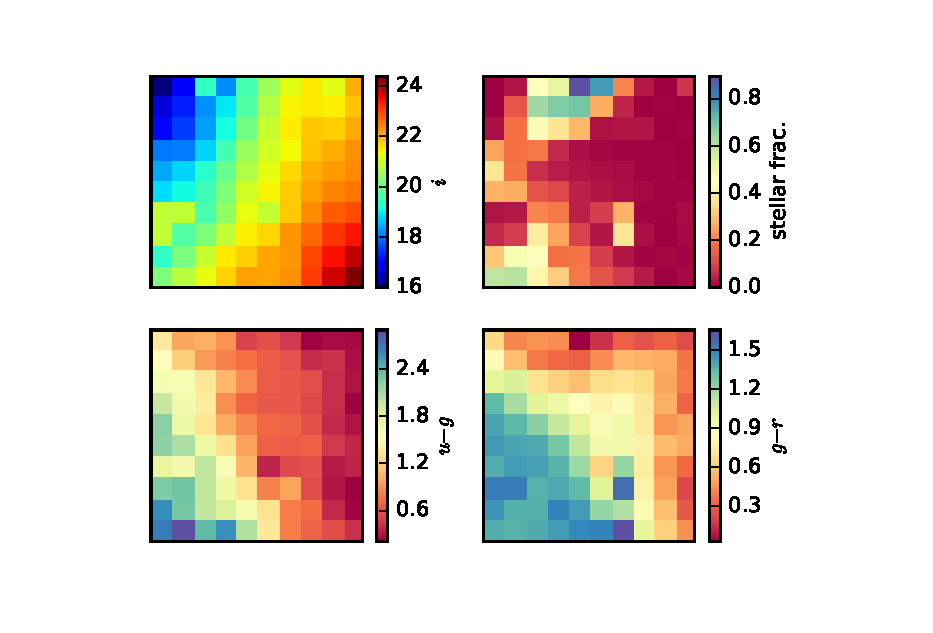
\includegraphics[width=\textwidth]{figures/som_colors.eps}
    \caption{A two-dimensional 10$\times$10 SOM representation
             showing the mean $i$-band magnitude (top left),
             the fraction of true stars in each cell (top right),
             and the mean values of $u-g$ and $g-r$
             for the cross validation data.}
    \label{fig:som_colors}
  \end{minipage}
  \hfill
  \begin{minipage}[t]{0.49\linewidth}
    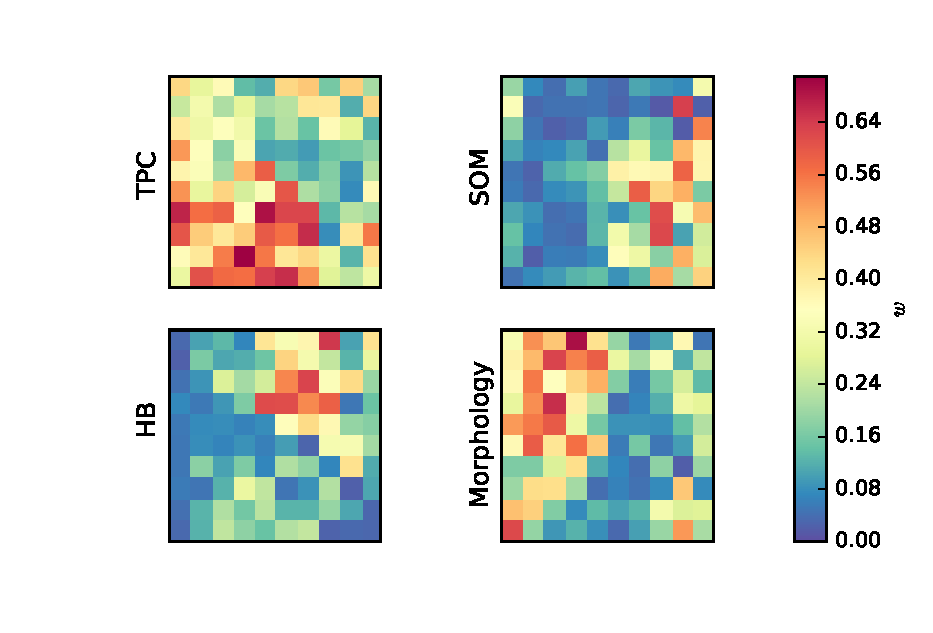
\includegraphics[width=\textwidth]{figures/weights.eps}
    \caption{A two-dimensional 10$\times$10 SOM representation
             showing the relative weights for the BMC combination technique
             applied to the four individual methods for the CFHTLenS data.}
    \label{fig:weights}
  \end{minipage}
\end{figure*}

In Figure~\ref{fig:som_colors}, we show
the mean CFHTLenS $i$-band magnitude in the top left panel
\textcolor{blue}{
and the fraction of stars in each cell in the top right panel.
}
The bottom two panels show the mean $u-g$ and  $g-r$ colors.
These two-dimensional maps clearly shows
the ability of the SOM to preserve relationships between sources
when it projects the full nine-dimensional space to the two-dimensional map.
The SOM mapping is a non-linear representation of all magnitudes and colors,
and thus these SOM maps should only be used to provide guidance.

We can also use the same SOM to determine the relative weights for 
the four individual classification methods for each cell.
We present the four weight maps for the BMC technique
in Figure~\ref{fig:weights}.
In these maps, a redder color indicates a higher weight,
or equivalently that the corresponding weight performs better in that region.
These weight maps demonstrate the variation in
the performance of the individual techniques across
the two-dimensional parameter space defined by the SOM.
Not surprisingly, the morphological separation
performs best in the top left corner of the $i$-band magnitude map,
which corresponds to the brightest CFHTLenS magnitudes $i \lesssim 20$.
On the other hand, \texttt{TPC} seems to perform best
in the region that corresponds to intermediate magnitudes
$20\gtrsim i \lesssim22.5$ and $1.5<u-g<3.0$.
Our unsupervised learning method \texttt{SOMc}
performs relatively better at fainter magnitudes $i>21.5$
with $0<u-g<0.5$ and $0<g-r<0.5$.
\textcolor{blue}{
Although \texttt{HB} shows the worst performance
when there exists ample training data,
BMC still utilizes information from \texttt{HB}
to produce an overall improvement in performance,
especially at intermediate magnitudes $20\gtrsim i \lesssim22$.
}

In Figure~\ref{fig:purity_mag}, 
we compare the star and galaxy purity values
for morphological separation, TPC, and BMC techniques
as a function of $i$-band magnitude.
Although morphological separation shows a slightly better performance
at bright magnitudes $i < 21$,
BMC outperforms both morphological separation and TPC
at faint magnitudes $i > 21$.
As shown in the histogram, the histogram peaks at $i \sim 22$,
and BMC therefore outperforms the morphological separation technique
for the majority of objects.
It is also clear that BMC outperforms TPC over all magnitudes.
BMC can accomplish this by combining information from
all base classifiers,
\eg giving more weight to the morphological separation method
at bright magnitudes.


\begin{figure*}
  \begin{minipage}[t]{0.49\linewidth}
    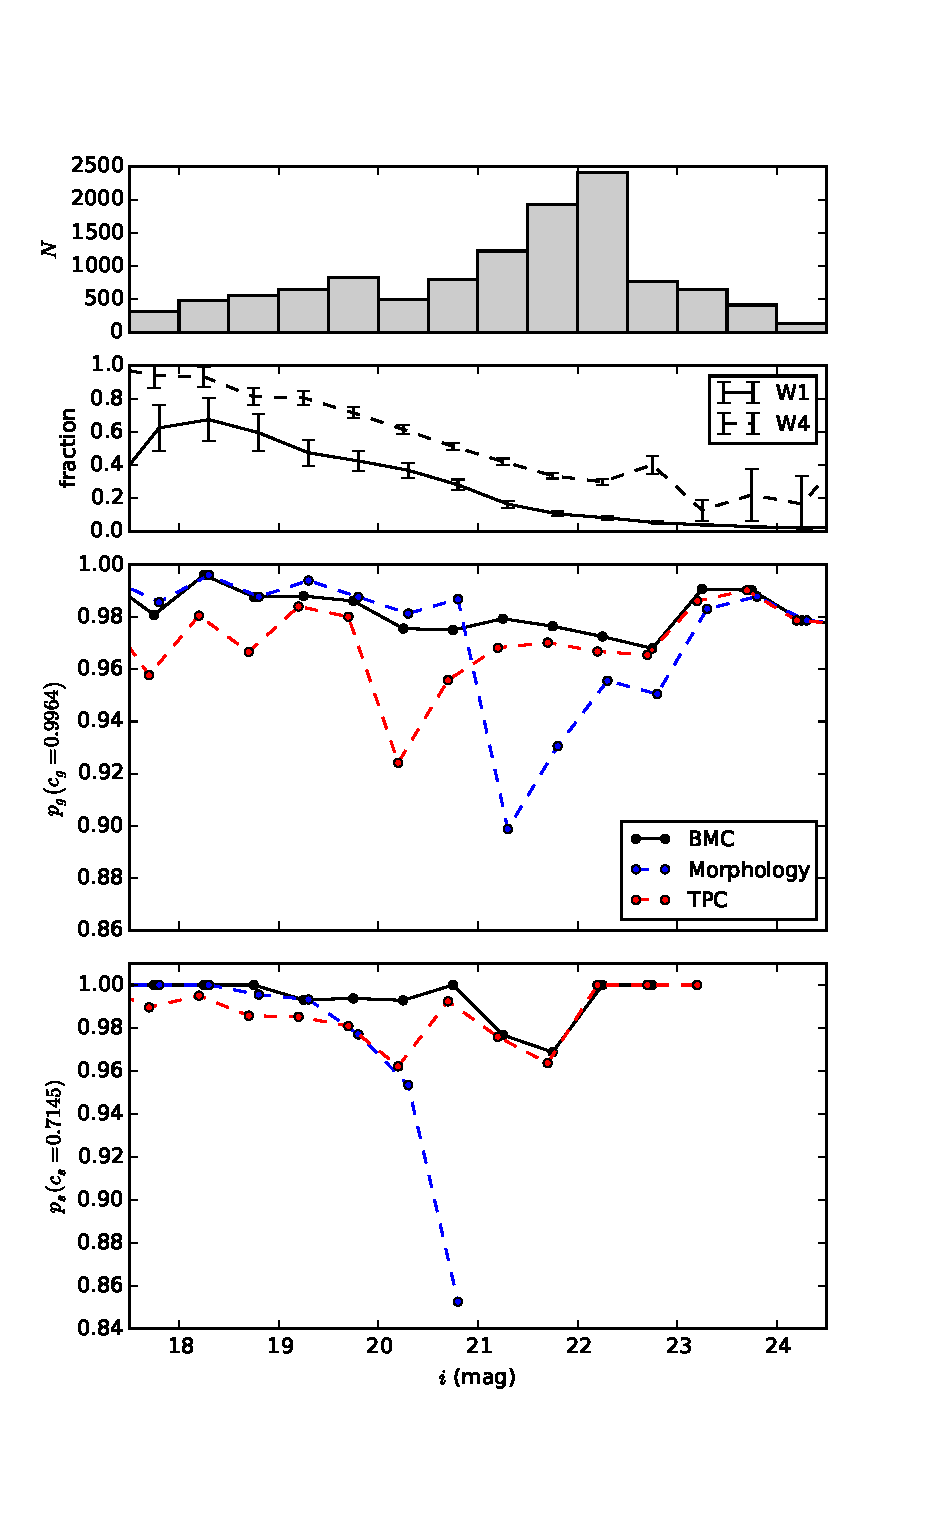
\includegraphics[width=\textwidth]{figures/purity_mag_cut.eps}
    \caption{Purity of morphological separation,
             TPC, and BMC techniques in 
             as a function of the $i$-band magnitude.
             The top panel shows the histogram of objects in the test data set.
             The second panel shows the fraction of stars
             as a function of magnitude. The error bars are Poisson.
             The bottom two panels compares
             the galaxy and star purity for morphological separation, TPC,
             and BMC techniques as a function of magnitude.
             The error bars for completeness and purity are not shown for
             clarity, but they are approximately 10 percent.}
    \label{fig:purity_mag_cut}
  \end{minipage}
  \hfill
  \begin{minipage}[t]{0.49\linewidth}
    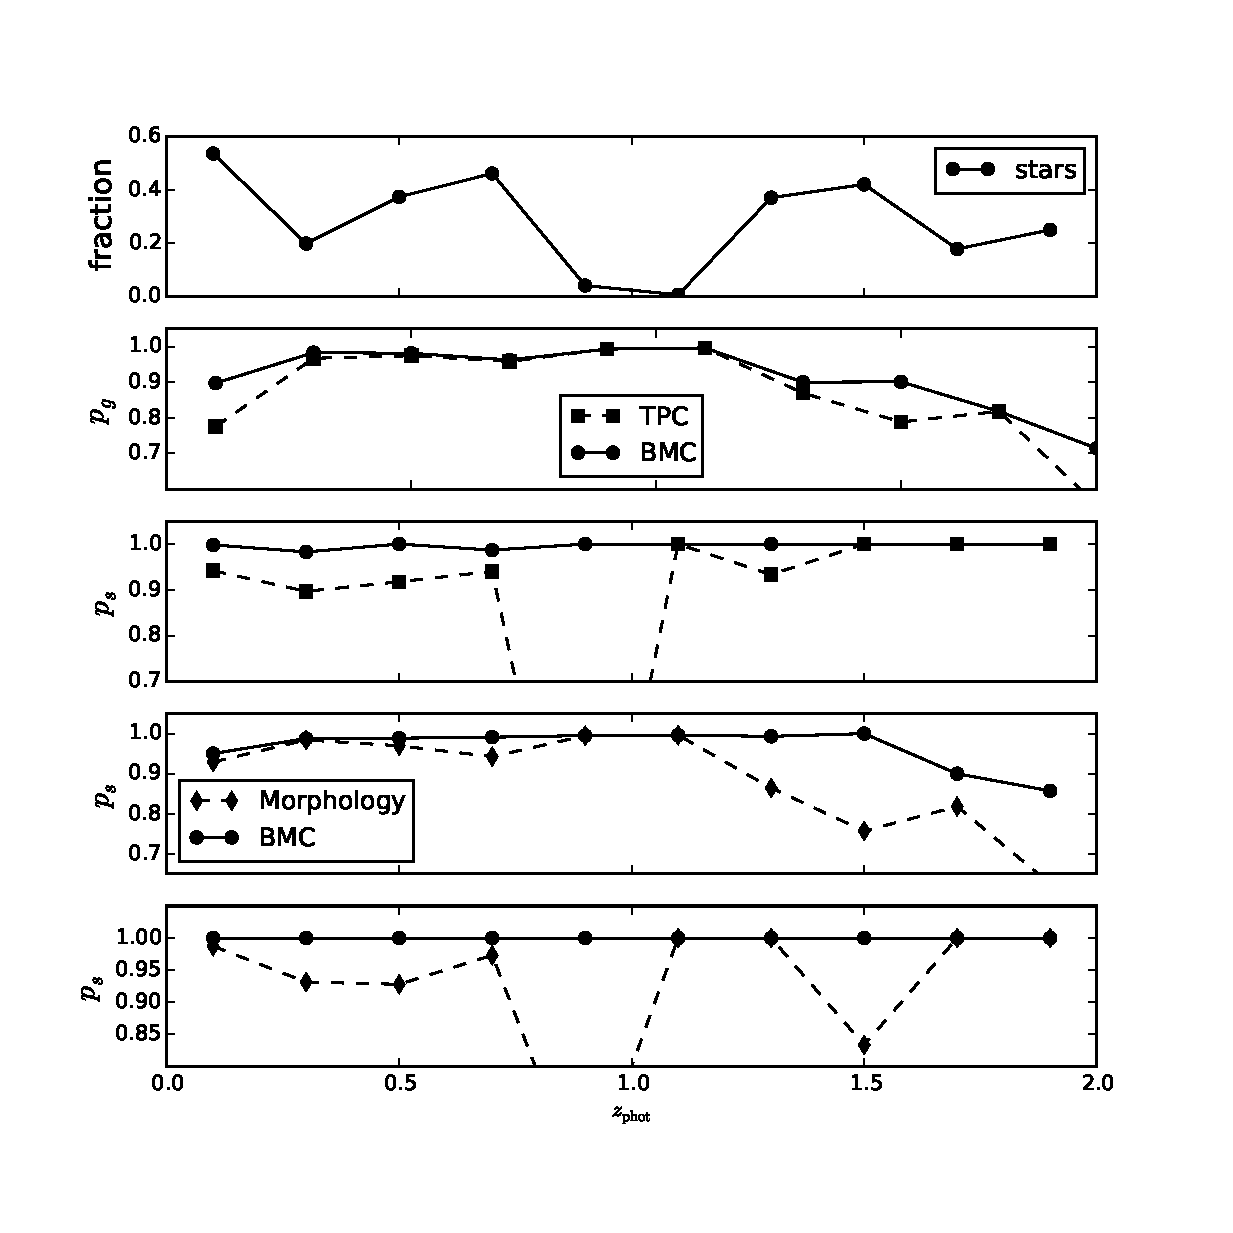
\includegraphics[width=\textwidth]{figures/purity_z.eps}
    \caption{The same figures as Figure~\ref{fig:purity_mag},
             but as a function of photometric redshift estimate
             (photo-$z$).}
    \label{fig:purity_z}
  \end{minipage}
\end{figure*}

\begin{figure}
%%  \begin{minipage}[t]{0.49\linewidth}
    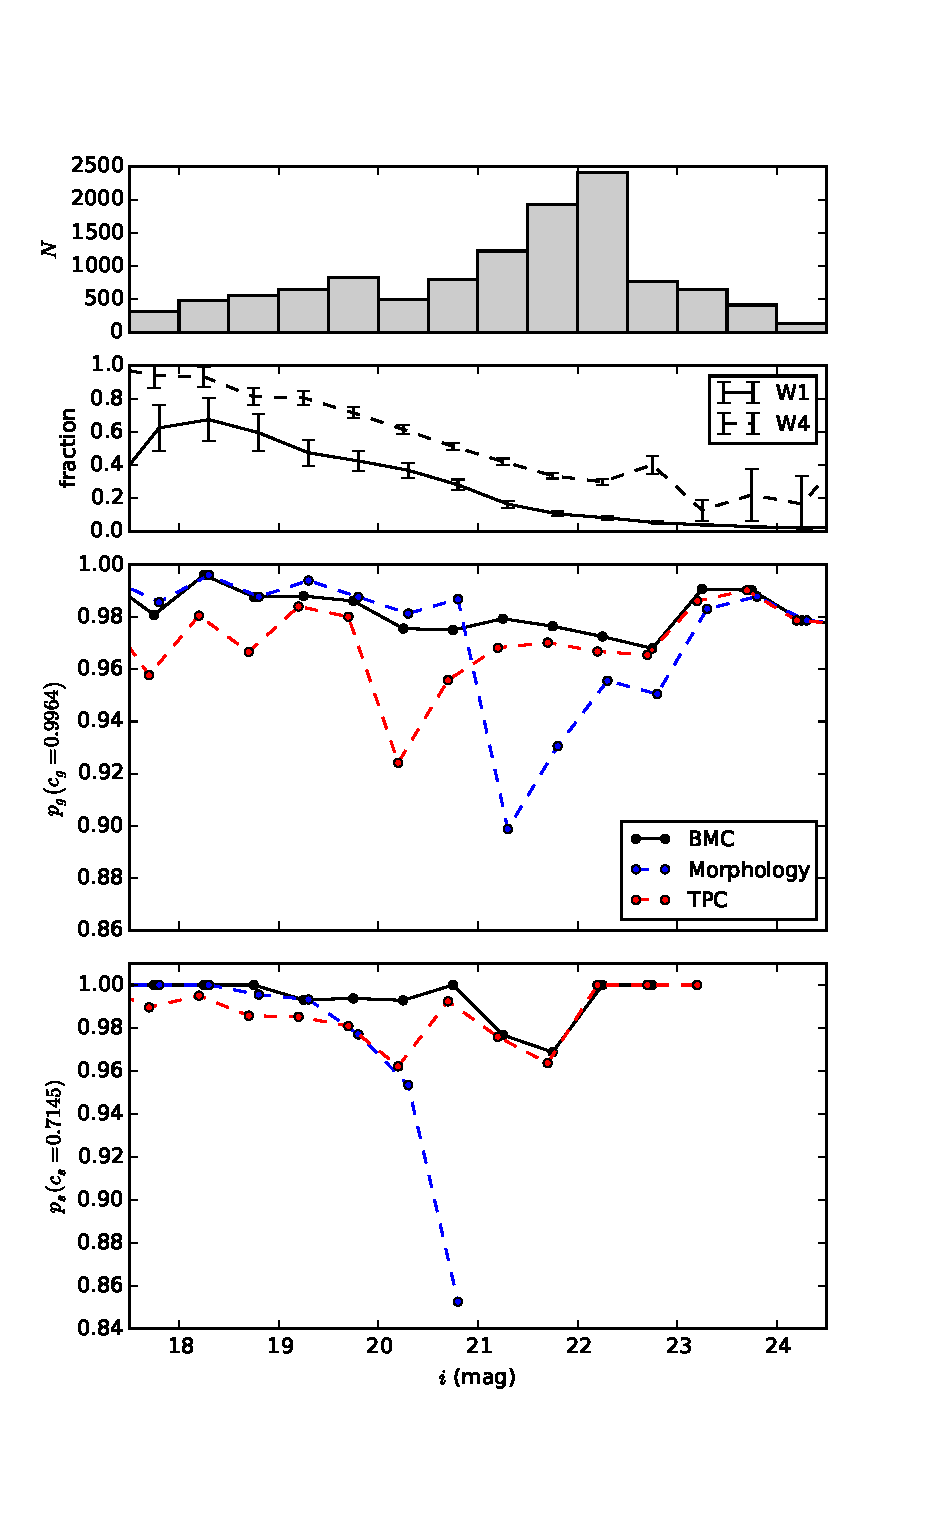
\includegraphics[width=\textwidth]{figures/purity_mag.eps}
    \caption{Purity of morphological separation,
             TPC, and BMC techniques in 
             Table~\ref{table:metrics_vvds}
             as a function of the $i$-band magnitude.
             The top panel shows the histogram of objects in the test data set.
             The second panel shows the fraction of stars
             as a function of magnitude. The error bars are Poisson.
             The bottom two panels compares
             the galaxy and star purity for morphological separation, TPC,
             and BMC techniques as a function of magnitude.
             The error bars for completeness and purity are not shown for
             clarity, but they are approximately 10 percent.
             }.
    \label{fig:purity_mag}
\end{figure}

\subsection{The Quality of Training Data}
  \label{section:quality_training}

It is very costly in terms of telescope time to
obtain a large sample spectroscopic observations
down to the limiting magnitude of a photometric sample.
Thus, we investigate the impact of training set quality
by imposing various magnitude and $z$ cuts
to decrease the size of the training set.

In Figure.~\ref{fig:perform_mag_cut}, we present
a visual comparison between different classification techniques
when various magnitude cuts are applied.

In Figure.~\ref{fig:perform_z_cut}, we also present
the result of imposing various $z$ cuts.

\begin{figure*}
  \begin{minipage}[t]{0.49\linewidth}
    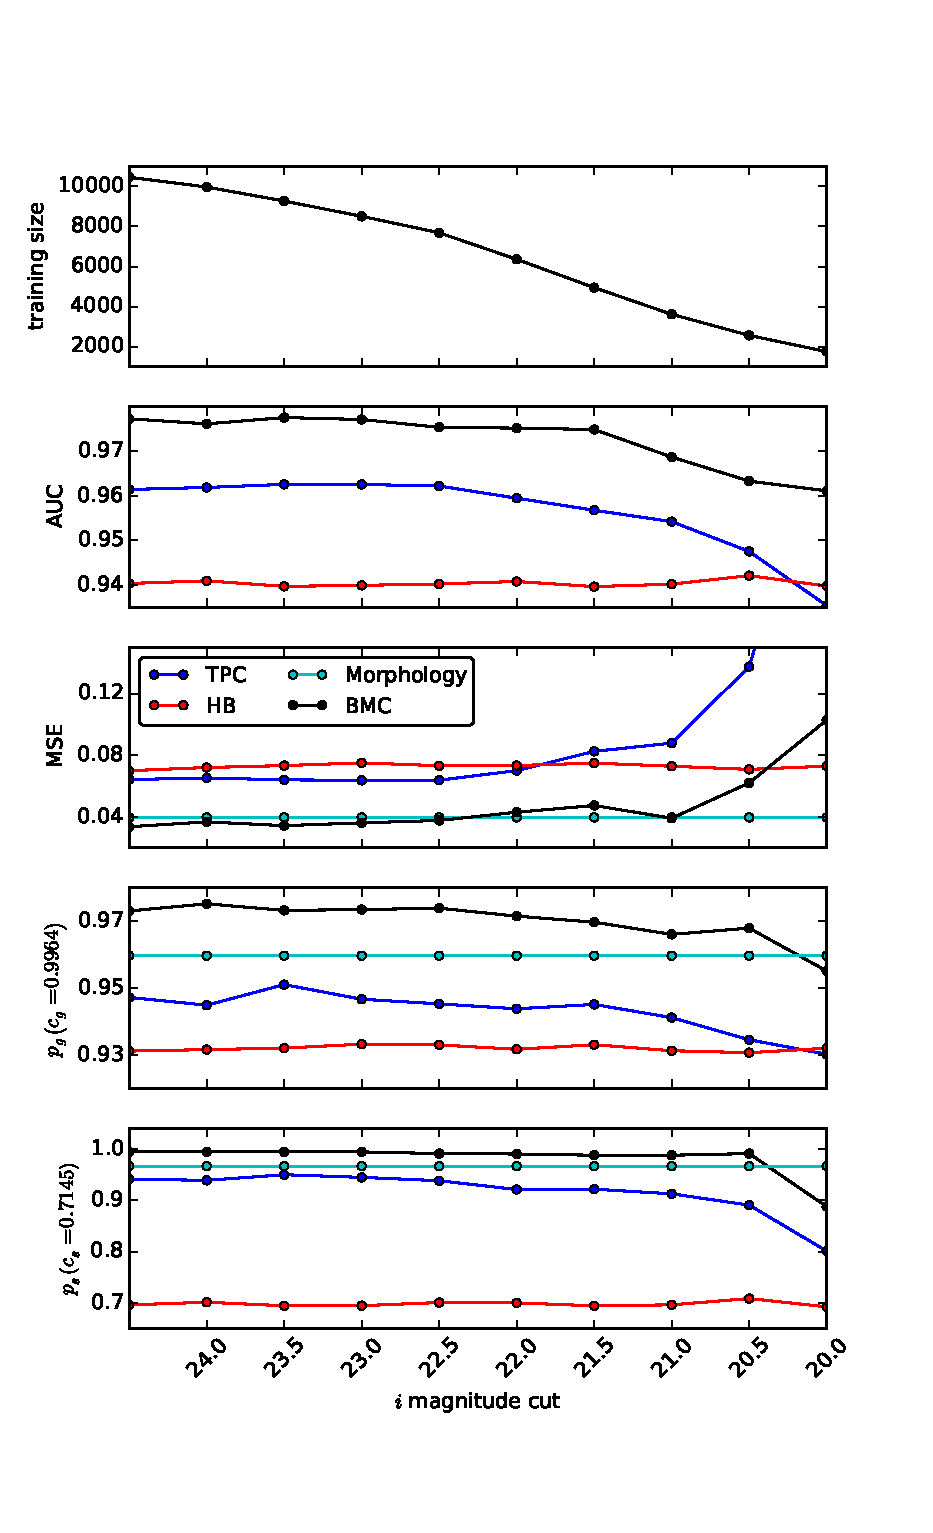
\includegraphics[width=\textwidth]{figures/perform_mag_cut.eps}
    \caption{The classification performance metrics for TPC, HB, morphology,
      and BMC as applied to the CFHTLenS data in the VVDS field
      with various magnitude cuts.
      The top panel shows the number of sources in the training set
      at corresponding magnitude cuts.
      We show only one of the four combination methods, BMC,
      which has the best overall performance.}
    \label{fig:perform_mag_cut}
  \end{minipage}
  \hfill
  \begin{minipage}[t]{0.49\linewidth}
    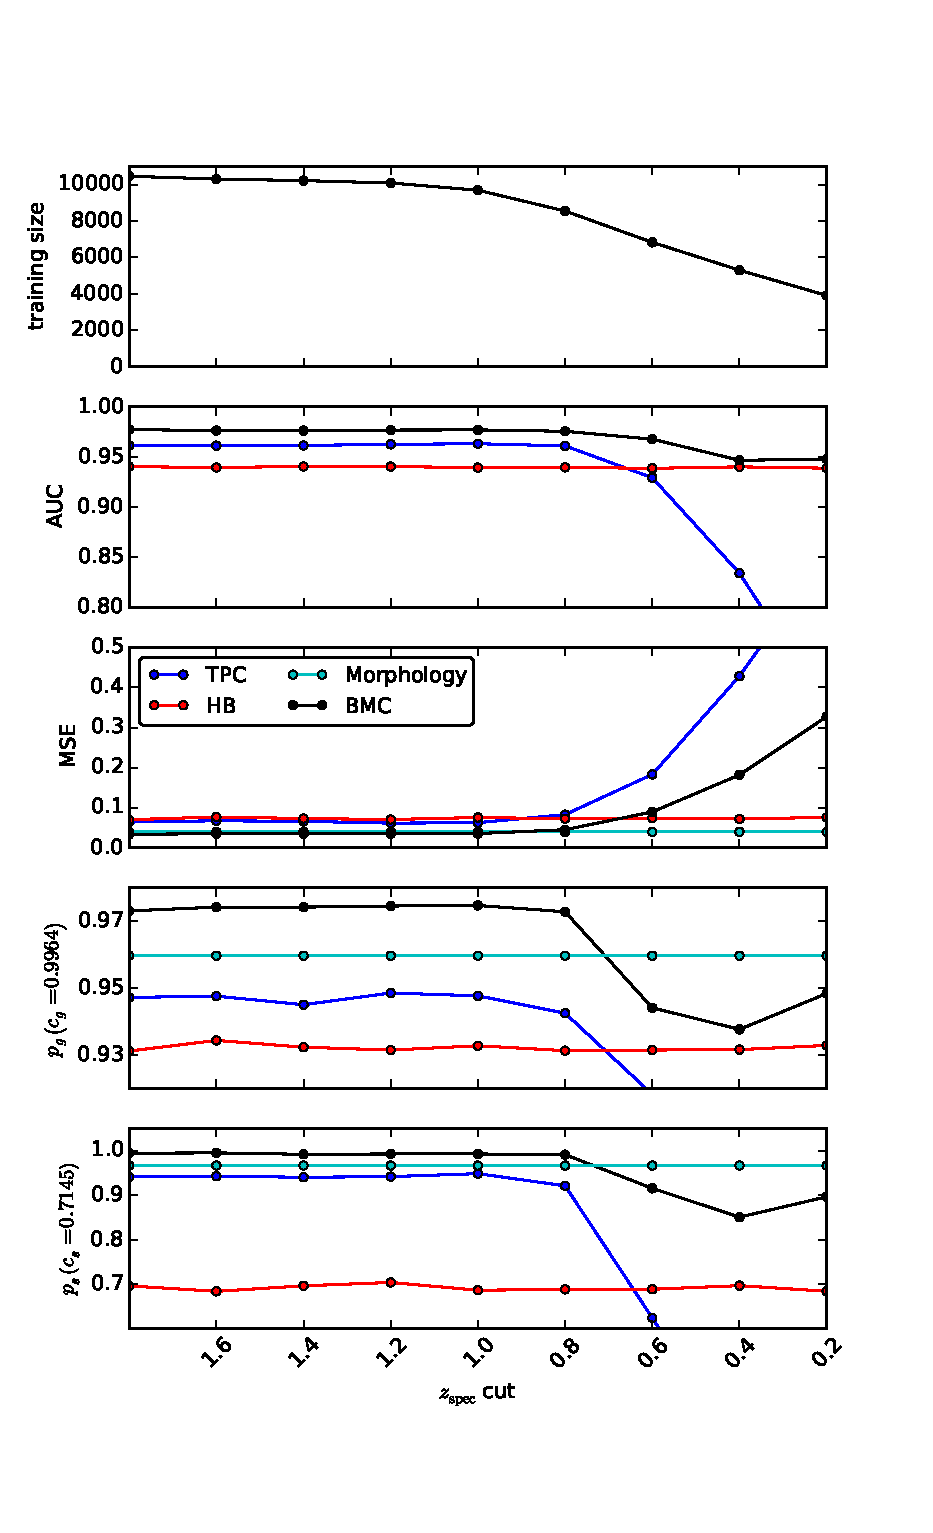
\includegraphics[width=\textwidth]{figures/perform_z_cut.eps}
    \caption{Same as Figure.~\ref{fig:perform_mag_cut} using
      $z_{\text{spec}}$ cuts.}
    \label{fig:perform_z_cut}
  \end{minipage}
\end{figure*}


\subsection{Insufficient Training Data}
  \label{section:poor_training}
  
We also investigate the impact of training set quality
by analyzing in detail a more realistic case
where the training data is available
only for a small number of objects at bright magnitudes.
To emulate this scenario,
we only use objects that have spectroscopic labels
from the VVDS 0226-04 field (which is located within the CFHTLS W1 field)
and impose a magnitude cut of $i < 22.0$ in the training data,
leaving us a training set with 1,365 objects.

\begin{table*}
  \caption{A summary of the classification performance metrics
           for the four individual methods
           and the four different classification combination methods
           as applied to the CFHTLenS data in the VVDS field
           with a magnitude cut of $i < 22.0$.
           The definition of the metrics is summarized in
           Table~\ref{table:metrics}.
           The bold entries highlight the best performance values
           within each column.}
  \centering
  \begin{tabular}{l c c c c c c}
    Classifier & AUC & MSE &
    $p_{g}\left(c_g=0.9964\right)$ & $p_{s}\left(c_s=0.7145\right)$ &
    $p_{g}\left(c_g=0.9600\right)$ & $p_{s}\left(c_s=0.2500\right)$\\
    \hline
    TPC  & 0.9601 & 0.0728 & 0.9438 & 0.9329 & 0.9819 & 0.9950\\
    SOMc & 0.9008 & 0.1679 & 0.8843 & 0.5044 & 0.9244 & 0.7726\\
    HB   & 0.8960 & 0.0894 & 0.9074 & 0.7516 & 0.9615 & 0.7793\\
    Morphology   & -      & \textbf{0.0397} & 0.9597 & 0.9666 & - & -\\
    WA   & 0.9639 & 0.0581 & 0.9613 & 0.9787 & 0.9756 & 1.0000\\
    BoM  & 0.9601 & 0.0728 & 0.9438 & 0.9329 & 0.9819 & 0.9950\\
    Stacking  & 0.9644 & 0.0613 & 0.9633 & 0.9835 & 0.9840 & 1.0000\\
    BMC  & \textbf{0.9738} & 0.0437 & \textbf{0.9676} & \textbf{0.9942} &
    \textbf{0.9878} & 1.0000\\
  \end{tabular}
  \label{table:metrics_vvds}
\end{table*}

We apply the same four star-galaxy classification techniques
and four different combination methods,
and test them on the same test data.
We present in Table~\ref{table:metrics_vvds}
the same six metrics for each method,
and highlight the best method for each metric.
Overall, the results obtained for the reduced data set are remarkable.
With poor training data, our data-driven methods,
\texttt{TPC} and \texttt{SOMc},
suffer a significant decrease in performance,
although they still in general perform better than 
the template fitting algorithm
\texttt{HB}.
The performance of our morphological separation method
does not depend on the training data,
and shows the best result in the MSE metric.
It also outperforms other base classifiers
in galaxy purity at galaxy completeness of 0.9964
and in star purity at star completeness of 0.7145.

Without sufficient training data,
the advantage of classification combination techniques
is more obvious.
Even WA, the simplest of combination techniques, outperforms
all individual classification techniques.
Interestingly, although TPC does not perform better
than morphological separation,
BoM still chooses TPC as the best model within each SOM cell
and shows exactly the same performance metrics as TPC.
Stacking and BMC techniques still outperform
all individual classification techniques,
and BMC's improvement in performance over TPC or mophological separation
is impressive.
Overall, the improvements are small but still significant
since these metrics are averaged over the full test data.


%% ROC curve for vvds i < 20
\begin{figure}
  \centering
  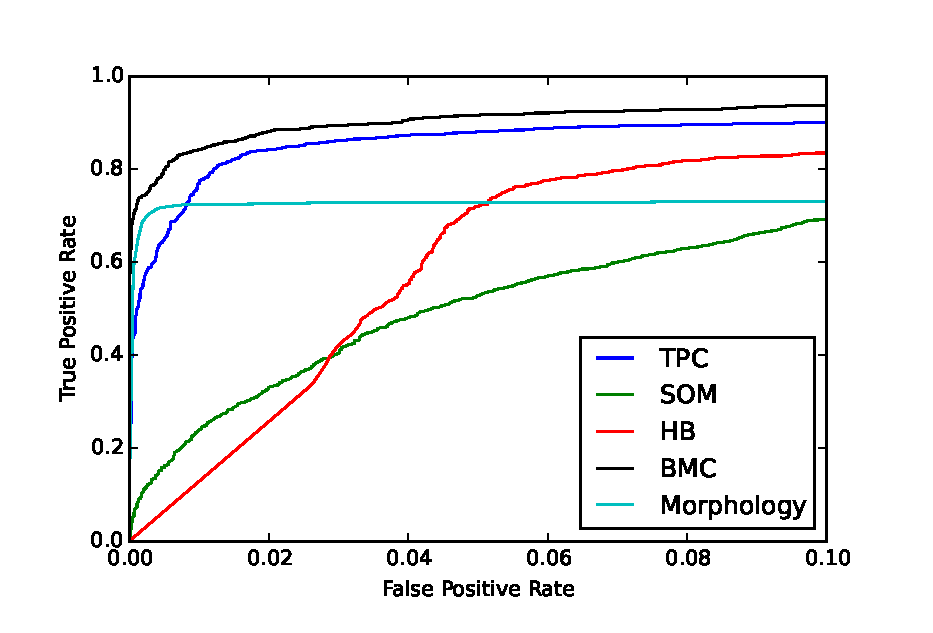
\includegraphics[width=\linewidth]{figures/roc_cut.eps}
  \caption{A magnified view of the ROC curve of
           four star-galaxy individual classification approaches
           (TPC, SOMc, HB, and morphology)
           and the best-performing combination technique (BMC).
           trained with the reduced data set.
           We show only one of the four combination methods, BMC,
           which has the best overall performance.}
  \label{fig:roc_cut}
\end{figure}

In Figure~\ref{fig:roc_cut}, we plot the ROC curve
of all four individual classification algorithm
and our BMC technique for the poor training data case.
We note that a binary classifier,
such as our cut-based morphological separation,
whose output is either zero or one,
is a single point in the ROC space.
We vary the half-light radius to create a smooth ROC curve
for morphological separation.
It is clear that our BMC technique dominates
each individual classification techniques in the ROC space.

%% weights map for vvds i < 20
\begin{figure}
  \centering
  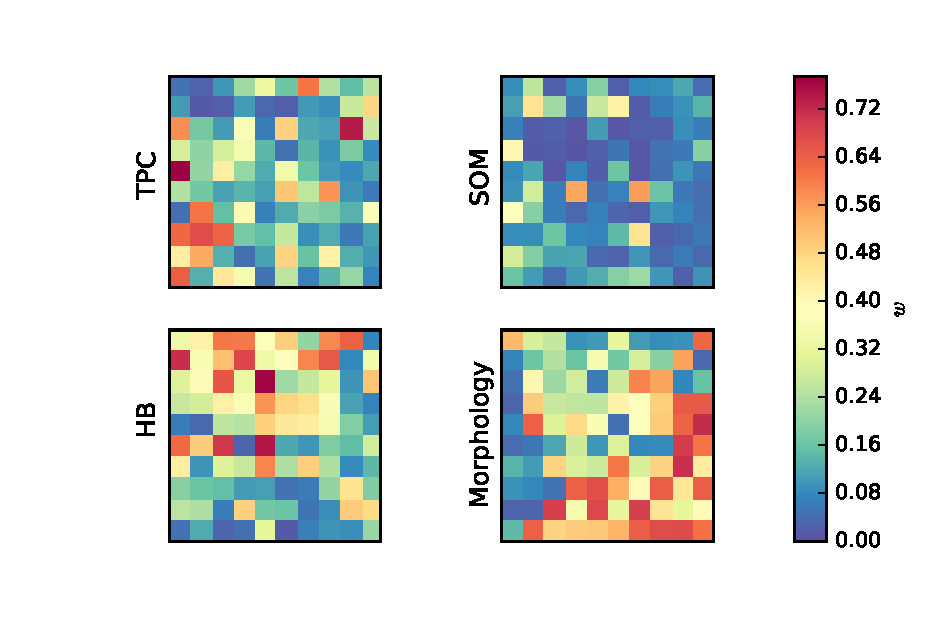
\includegraphics[width=\linewidth]{figures/weights_cut.eps}
  \caption{A two-dimensional 10$\times$10 SOM representation
           showing the relative weights for the BMC combination technique
           applied to the four individual methods
           trained with the CFHTLenS data in the VVDS field
           with $i < 22$.}
  \label{fig:weights_cut}
\end{figure}

In Figure~\ref{fig:weights_cut}, we again show the $10\times10$
two-dimensional weight map defined by the SOM.
It seems that \texttt{TPC} performs well
in most of the parameter space.
When the quality of training data is relatively poor,
the performance of data driven algorithms will decrease,
while the performance of template fitting algorithms such as \text{HB}
is independent of training data.
Thus, it is perhaps not surprising that
BMC algorithm now uses information from \texttt{HB},
whereas it assigned almost no weight to \texttt{HB}
when we had a high-quality training data.
Another interesting pattern is that
\texttt{SOMc} and morphological separation seem complementary;
\texttt{SOMc} is weighted most strongly at fainter magnitudes,
while the morphological separation method
is weighted most strongly at brighter magnitudes.
It is not surprising that the morphological separation method
performs best at bright magnitudes,
and BMC uses almost no morphological information at faint magnitudes.


\begin{figure*}
  \begin{minipage}[t]{0.49\linewidth}
    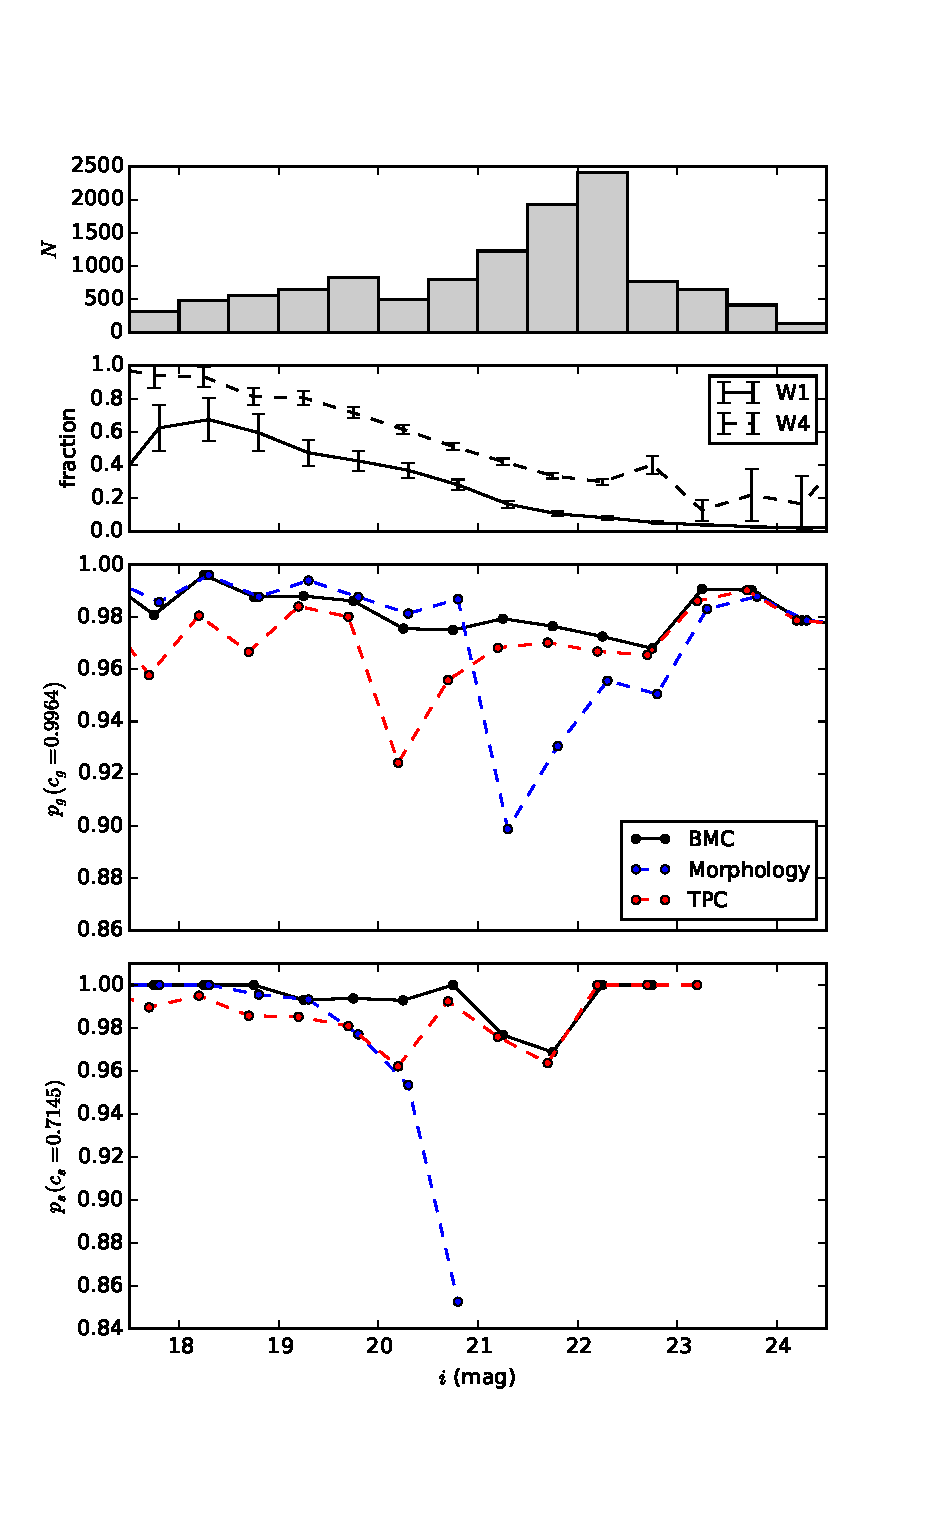
\includegraphics[width=\textwidth]{figures/purity_mag_cut.eps}
    \caption{Purity of morphological separation,
             TPC, and BMC techniques in 
             Table~\ref{table:metrics_vvds}
             as a function of the $i$-band magnitude.
             The top panel shows the fraction of stars
             as a function of magnitude.
             the galaxy and star purity for TPC and BMC techniques.
             The bottom two panels show
             the galaxy and star purity for morphological separation
             and BMC technique.
             We use the same threshold values from 
             Figure~\ref{fig:purity_mag} in the bottom four panels}.
    \label{fig:purity_mag_cut}
  \end{minipage}
  \hfill
  \begin{minipage}[t]{0.49\linewidth}
    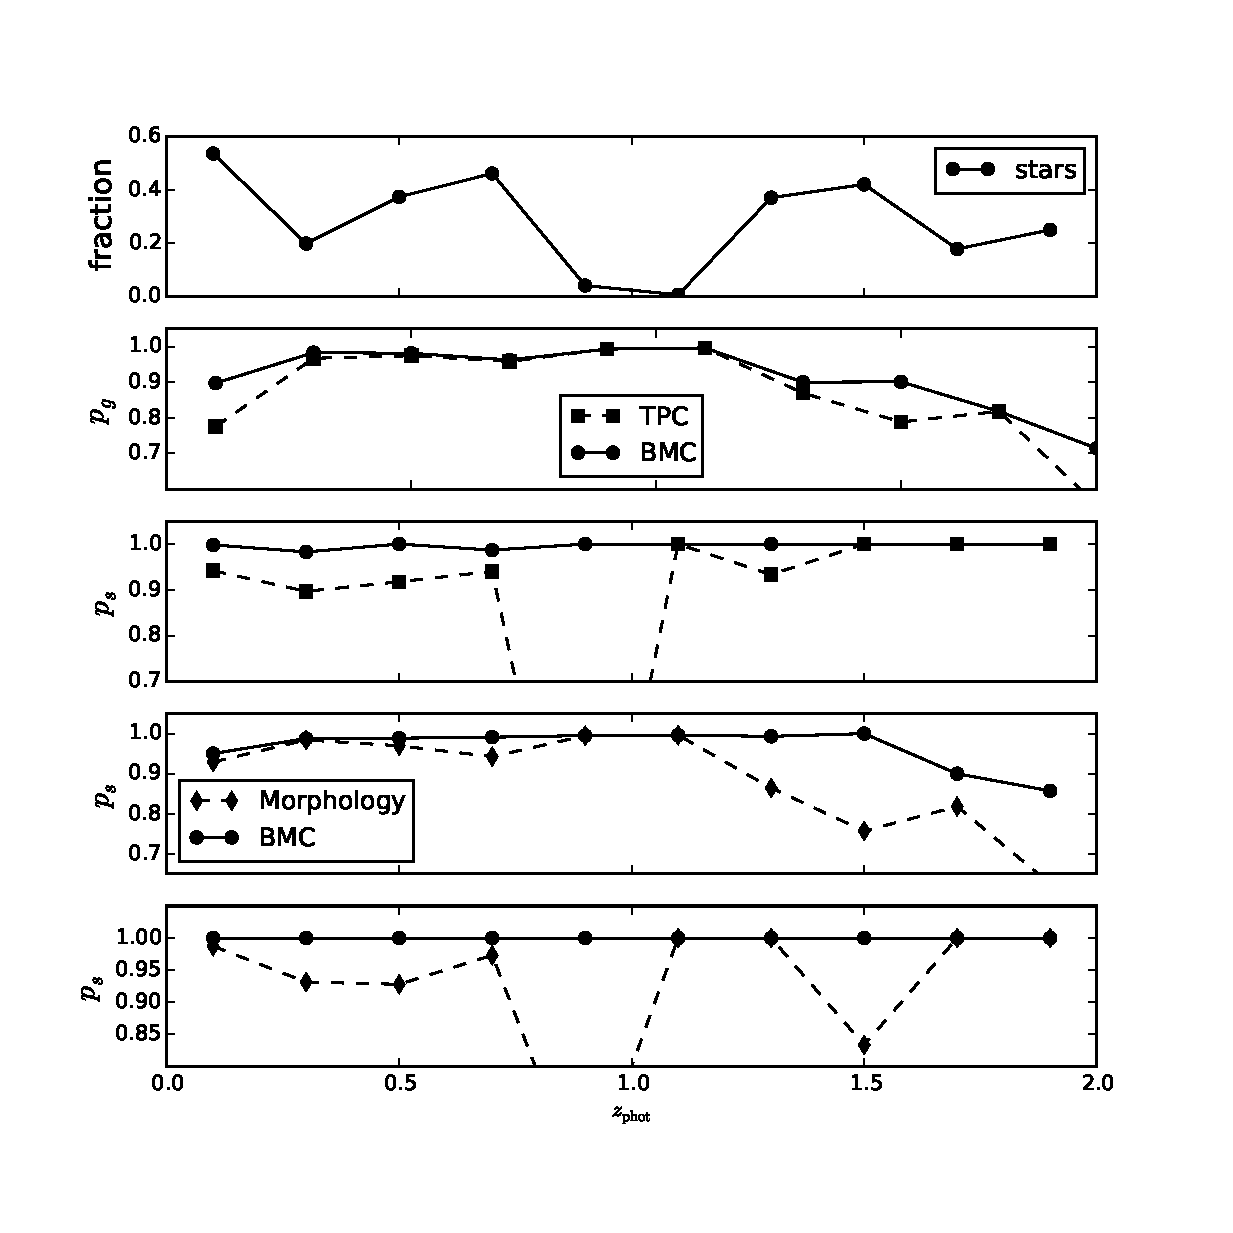
\includegraphics[width=\textwidth]{figures/purity_z.eps}
    \caption{The same figures as Figure~\ref{fig:purity_mag},
             but as a function of photometric redshift estimate
             (photo-$z$).}
    \label{fig:purity_z}
  \end{minipage}
\end{figure*}

We present the star and galaxy purity values
of Table~\ref{table:metrics_vvds} as a function of
$i$-band magnitude in Figure~\ref{fig:purity_mag}.
It is clear that BMC outperforms both
morphological separation and TPC classification techniques
over all magnitudes.
The galaxy purity of BMC is significantly better
than that of TPC at bright magnitudes, $i\lesssim21.5$,
while they are similar at faint magnitudes.
The star purity of BMC shows improvement over that of TPC
at faint magnitudes,
while they are similar at bright magnitudes.
As suggested by the weight maps in Figure~\ref{fig:weights_cut},
BMC can accomplish this by combining information from
all base classifiers,
\eg giving more weight to the morphological separation method
at bright magnitudes.
We can also see in the bottom two panels that
the performance of morphological separation suffers
at intermediate magnitudes $21\lesssim i \lesssim23$,
while BMC shows consistently better performance
over all magnitude ranges.


We also show the star and galaxy purity values
of Table~\ref{table:metrics_vvds} as a function of
photometric redshift in Figure~\ref{fig:purity_z}.
Photo-$z$ is estimated with
the \texttt{BPZ} algorithm~\citep{benitez2000bayesian}
and provided with
the CFHTLenS photometric redshift catalogue~\citep{Hildebrandt2012}.
It is again clear that BMC outperforms
both individual classification techniques over all redshift range.

\begin{figure*}
  \begin{minipage}[t]{0.49\linewidth}
    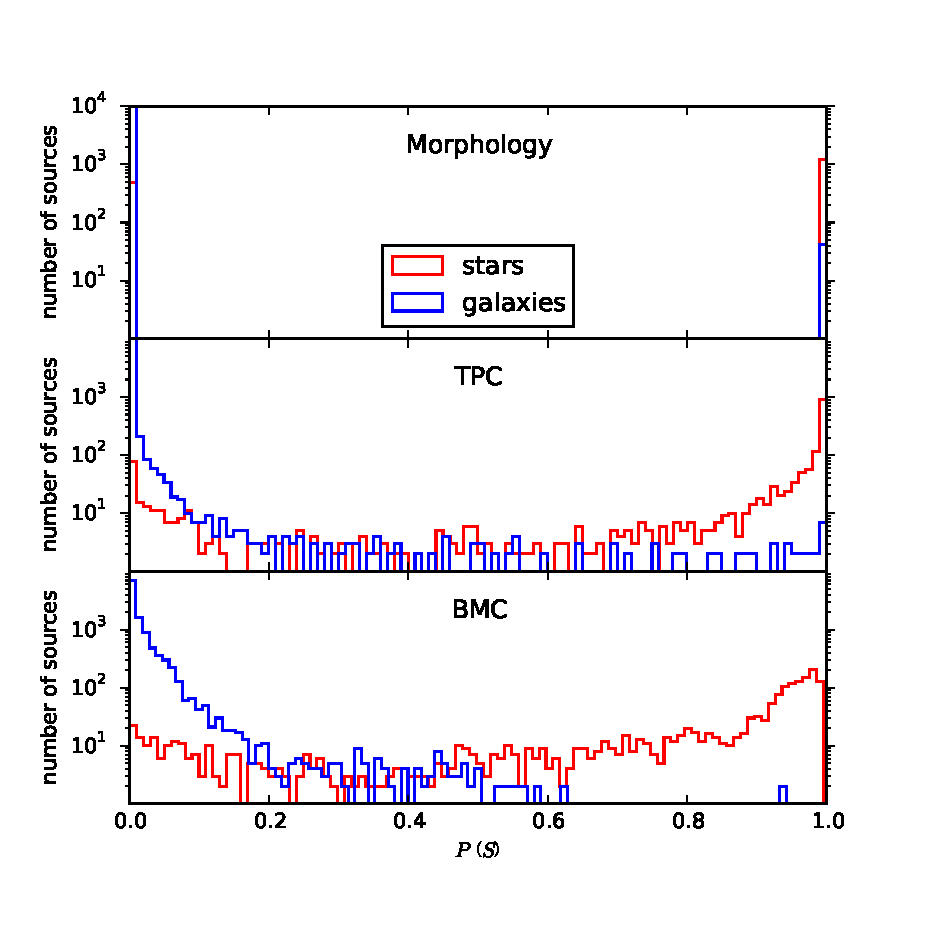
\includegraphics[width=\textwidth]{figures/p_dist_all.eps}
    \caption{Histogram of the posterior probability that
             a source is a star for morphological separation (top),
             TPC (middle), and BMC (bottom) techniques
             for the entire training data
             (the CFHTLenS data in the DEEP2, SDSS, VIPERS, and VVDS
             fields as discussed in Section~\ref{section:rich_training}).}
    \label{fig:p_dist_all}
  \end{minipage}
  \hfill
  \begin{minipage}[t]{0.49\linewidth}
    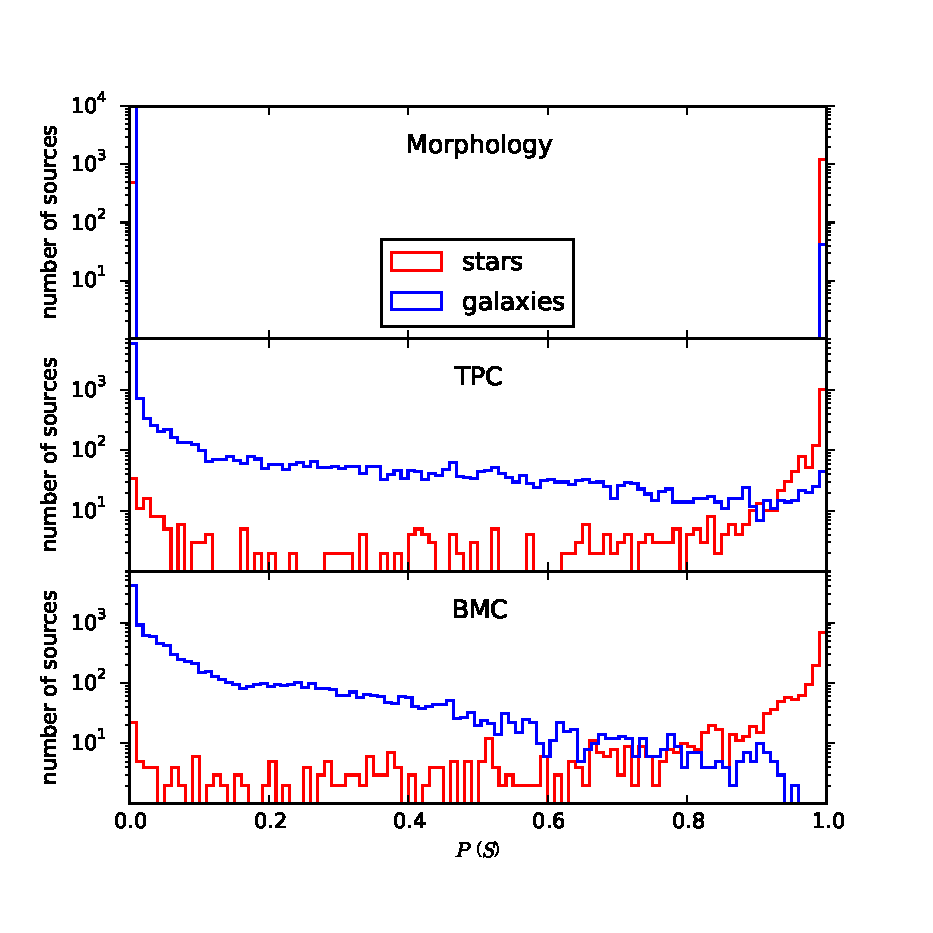
\includegraphics[width=\textwidth]{figures/p_dist_cut.eps}
    \caption{The same figures as Figure~\ref{fig:p_dist_all},
             but for TPC and BMC trained with 
             poor training data
             (the CFHTLenS data in the VDDS field
             with a magnitude cut of $i<22$).}
    \label{fig:p_dist_cut}
  \end{minipage}
\end{figure*}

We show the distribution of posterior star probabilities
in Figures~\ref{fig:p_dist_all} and \ref{fig:p_dist_cut}.
The histogram of spectroscopic galaxies is in blue,
and the histogram of true stars is in red.
It is interesting that the BMC technique assigns
a probability $P\left(S\right)$ greater than 0.6
to almost no true galaxies in Figure~\ref{fig:p_dist_all},
presumably because BMC utilizes information from
different types of classification techniques.
This pattern is more pronounced in Figure~\ref{fig:p_dist_cut},
where the $P\left(S\right)$ distribution of BMC for true galaxies
falls off sharply at $P\left(S\right)\approx0.95$,
while morphological separation and TPC techniques
classify some true galaxies as stars with absolute certainty.


\begin{figure*}
  \centering
  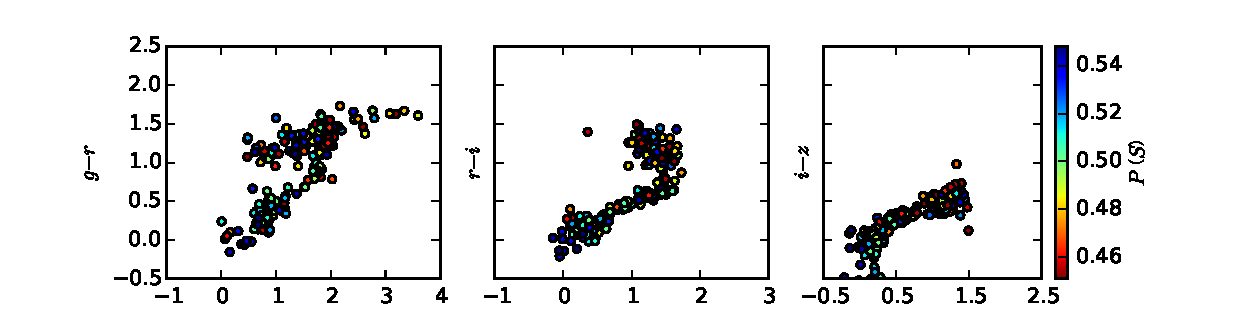
\includegraphics[width=\linewidth]{figures/color_color.eps}
  \caption{Color-color diagrams of sources with
           $0.45<P\left(S\right)<0.55$ when the BMC technique
           is applied to the poor training data.}
  \label{fig:color_color}
\end{figure*}

To identify the regions in color-color space
where our BMC technique struggles to classify stars and galaxies,
we present the distribution over the color-color space for sources with
$0.45 < P(S) < 0.55$ in Figure~\ref{fig:color_color}.
Not surprisingly, these regions correspond to
where there is a significant overlap between stars and galaxies
in the color space.
It may be possible to improve the performance of
star-galaxy classification by obtaining more information
through spectroscopic follow-up, manual study, or citizen science projects,
or by developing a classification technique specifically designed
for these regions of the color space and
combining it with other techniques in a Bayesian framework.

\section{Conclusions}
  \label{section:conclusions}

\textcolor{blue}{begin new text}

We have presented and analyzed a novel star-galaxy classification framework
for combining classifications from the CFHTLenS project.
In particular, we use four independent star-galaxy classification techniques:
a morphological separation method;
\texttt{TPC}, a supervised machine learning technique
based on prediction trees and a random forest;
\texttt{SOMc}, an unsupervised machine leraning approach
based on self-organizing maps and a random atlas;
and \texttt{HB}, a hierarichical bayesian template-fitting method
that we have modified and parallized.
Both \texttt{TPC} and \texttt{SOMc} are currently availble within
a software package named
\texttt{MLZ}\footnote{http://lcdm.astro.illinois.edu/code/mlz.html}.
Our implementaion of \texttt{HB} and \texttt{BMC},
as well as IPython notebooks that were used to
produce the results in this paper,
are available at \url{https://github.com/EdwardJKim/astroclass}.

\textcolor{blue}{end new text}

When there's wealth of training data,
TPC is so good that combination techniques show
no significant improvement over TPC.

Even with poor (but reasonable) training data,
TPC outperforms unsupervised methods.

In a more realistic case where the training data is poor,
BMC should be used.

Probabilistic classification is better.
Binary classification can be transformed into a probabilistic
classification when combined with other models in a Bayesian framework.

We note that \cite{carrascokind2014exhausting} analyzed
different techniques for combining
photometric redshift probability density functions (photo-$z$ PDFs),
and also found that BMC is in general the best
photo-$z$ PDF combination technique.

\textcolor{red}{more here}

\section*{Acknowledgements}

We thank the referee for a careful reading of the manuscript
and comments that improved this work.
We thank Ignacio Sevilla for helpful and insightful conversations.
We acknowledge support from the National Science Grant No.
\textcolor{red}{XXXX}.

We gratefully acknowledge the use of computing resources
from the Extreme Science and Engineering Discovery Environment (XSEDE),
which is supported by National Science Foundation grant number
\textcolor{red}{XXXX}.

Funding for CFHTLenS has been provided by
\textcolor{red}{XXXX}.

\bibliographystyle{mn2e}

\bibliography{sg_paper}

\bsp

\label{lastpage}

\end{document}
